
\chapter{Implementation}
\label{sec:implementation}
\noindent

\noindent In this chapter, we provide a detailed implementation of our proposed methodology. We start with presenting the software platform we incorporated to shape and design. Then we demonstrate our network's architecture in detail. Finally, we attempt to give insight into the datasets we used to train and test our model. 

\section{Caffe deep learning platform}

Caffe is a clean and modifiable framework for state-of-the-art deep learning algorithms and a collection of reference models. The framework is a BSD-licensed C++ library with Python and MATLAB bindings for training and deployment of general-purpose convolutional neural networks and other deep models on commodity architectures \cite{jia2014caffe}. It powers on-going research projects and large-scale industrial applications in vision, speech and multimedia by CUDA \footnote{CUDA is a parallel computing platform and application programming interface (API) model created by NVIDIA \cite{cuda}, processing over 40 million images a day on a single K40 or Titan GPU \cite{jia2014caffe}.}  GPU computation.
The main components of Caffe architecture are outlined below:
\begin{enumerate}

\item \textbf{Data storage:} Caffe stores and communicates data in 4-dimensional arrays called \textit{blobs}. Blobs provide a unified memory interface, holding batches of data, parameters, or parameter updates. Blobs conceal the computational overhead by synchronizing from the CPU host to the GPU device as needed. Caffe supports some data sources such as LevelDB or LMDB (Lightning Memory-Mapped Database), HDF5, MemoryData, ImageData, etc. However, large-scale data is stored in LevelDB databases since it reads the data directly from memory\cite{caffe}. 
\item \textbf{Layers:} A caffe layer takes blobs as input and yields one or more as output. In a network(as described in chapter~\ref{subsec:bp}), each layer plays two important roles: a forward pass that takes the inputs and produces the outputs, and a backward pass that takes the gradient with respect to the output, and computes the gradients with respect to the parameters and to the inputs, which are in turn back-propagated to earlier layers \cite{jia2014caffe}.

\indent Caffe supports an exhaustive set of layers, including the following\cite{jia2014caffe}: 
\begin{enumerate}
	\item convolution, pooling, fully connected, 
	\item nonlinearities like rectified
	linear and logistic, local response normalization, element-wise operations, and 
	\item losses like softmax and hinge
\end{enumerate}
\item \textbf{Networks and run mode:} Caffe ensures the correctness of the forward and backward passes for any directed acyclic graph of layers. A typical network begins with a data layer laying at the bottom going up to the loss layer that computes tasks' objectives. The network is ran on CPU or GPU independent of the model definition. 
\item \textbf{Training a network:} Training phase in Caffe is done by classical stochastic gradient descent algorithm. When training, images and labels pass through different layers lead into the final prediction into a classification layer that produces the loss and gradients which train the whole network. Figure~\ref{fig:caffe} illustrates a typical example of a Caffe network. 


\indent Finetuning, the adaptation of an existing model to new architectures or data, is a standard method in Caffe. Caffe  finetunes the old model weights for the new task and initializes new weights as needed. This capability is essential for tasks such as knowledge transfer \cite{donahue2013decaf}, object detection \cite{girshick2014rich}, and object retrieval \cite{guadarrama2014open} \cite{jia2014caffe}.  
\end{enumerate}

\begin{figure}[H]
	\centering
	{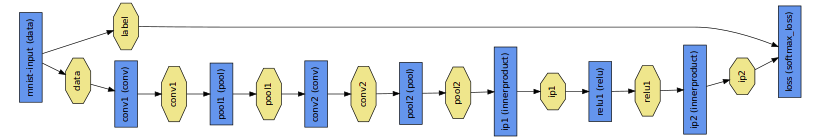
\includegraphics[width=1\textwidth]{images/caffe}}
	\caption{An MNIST digit classification example of a Caffe network, where blue boxes represent layers and yellow octagons represent data blobs produced by or fed into the layers\cite{jia2014caffe}.}
	\label{fig:caffe}
\end{figure}

\textbf{Justification}. We decided to use Caffe because, it addresses computation efficiency problems (as likely the fastest available implementation of deep learning frameworks at the time of performing this study, adheres to software engineering best practices, providing unit tests for correctness and experimental rigor and speed for deployment. It is also well-suited for research use, due to the well-implemented modularity of the code, and the clean separation of network definition (usually the novel part of deep learning research) from actual implementation\cite{jia2014caffe}. In addition, it provides a python wrapper which exposes the solver module for easy prototyping of new training procedures. 

\section{The architecture}
\label{imparch}
In learning features or object representations for vision tasks and by the use of neural networks, the depth of network plays an important role. The deeper the model, the better it learns. However, issues like overfitting and underfitting should not be left neglected.   
Having Caffe platform introduced, we propose the designed network for two experiments we did regarding learning to count problems. Therefore, in this section, networks' settings and architectures for even digit recognition and crowd counting problems will be described separately. 

\subsection{Even digit recognition}
\label{subsubsec:digitarch}
For learning to count even digits problem, since we used MNIST dataset to generate our dataset, we decided to start with an architecture similar to the classic MNIST hand-written digit recognition problem\cite{lecun1995comparison}. From there, we modified the architecture to optimize the performance of the network.

\indent In our network, the data layer fetches the images and labels from the disk, passes it through, the first convolutional layer with 20 filters, each of size $15\times15$ followed by a ReLU non-linearity and LRN normalization layer. Then the output is pooled by the size of $2\times2$. This process repeats again but this time with the second convolutional layer having 50 filters of size $3\times3$. In all convolution and pooling layers, the \textit{stride} = 1 and \textit{padding} = 1 are considered (see section~\ref{convlayer} for more explanation regarding padding and stride). 
\begin{wrapfigure}[45]{r}{0.58\textwidth}
  \centering
   {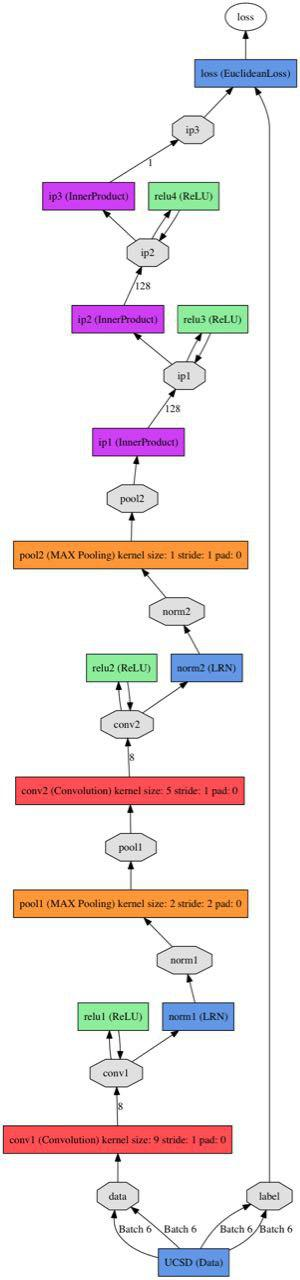
\includegraphics[width=0.33\textwidth]{images/model}}
  %\end{center}
	\caption{Proposed network architecture for the  Even digits recognition task}
	\label{fig:l2cNet}
\end{wrapfigure}

\noindent the output of the second pooling layer is fed to two fully connected (inner product) layers with respectively 64 and 1 number of outputs (since the problem is approached as a regression task). Both fully connected layers are followed by ReLU non-linearities. Figure~\ref{fig:l2cNet} shows a schematic of the architecture. In addition, parameters of the network are set as below:
\begin{itemize}
\item \textbf{Learning rate:} The basic learning rate is 0.0001. However, for our experiment we chose \textit{multi-step} learning policy in which, after each \textit{stepsize}=40000 iterations, the learning rate drops by the rate of $\gamma = 0.1$. This initialization is based on rule of thumb used in \cite{krizhevsky2012imagenet}.
\item \textbf{Momentum:} We use momentum $\mu = 0.9$. This selection also is based on the rule of thumb. As momentum value $\mu$ effectively multiplies the size of our updates by a factor of $\frac{1}{1-\mu}$. Hence, changes in momentum and learning rate ought to be accompanied with an inverse correlation. When momentum $\mu = 0.9$, we have an effective update size of 10 since we also drop the learning rate by the factor of $\gamma= 0.1$.
\item \textbf{Weight decay:} Weight decay as a penalty term to the error function, has a constant value of 0.0005. This decay constant is multiplied to the sum of squared weights.
\end{itemize}

\noindent We should also mention that at the top layer of the network, we used \textit{Euclidean Loss }layer to compute  the euclidean distance between the predictions and the ground truth. 

\begin{wrapfigure}[44]{r}{0.58\textwidth}
  \centering
   {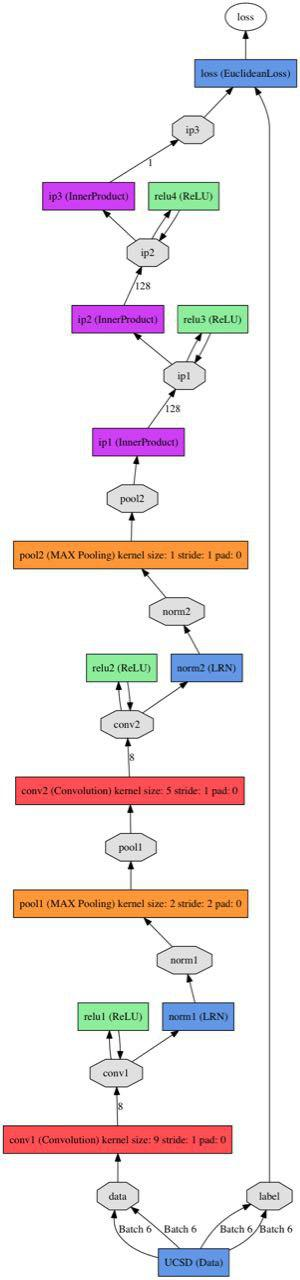
\includegraphics[width=0.31\textwidth]{images/model}}
  %\end{center}
	\caption{Proposed network architecture for Even digits recognition task}
	\label{fig:l2cNet}
\end{wrapfigure}
%\newpage
\subsection{Crowd counting}
\label{subsec:ucsdarch}
In the case of counting pedestrians task, we applied the same settings to a different architecture. This time, due to more complexity of images, we considered a deeper network. Here the data blobs pass through 4 convolutional layers. First convolutional layer has 4 filters, each with $5\times5$ kernel and the other 3 layers have again 4 filters but each of size $3\times3$. Similar to the previous model, each convolutional layer is followed by ReLU non-linearity layer and LRN normalization layer. Also the stride and padding values for all the convolutional layers are respectively equal to 1 and 0. 

In the case of counting pedestrians task, we applied the same settings to a different architecture. This time, due to higher complexity of images, we considered a deeper network. Here the data blobs pass through 4 convolutional layers. First convolutional layer has 4 filters, each with 5*5 kernel and the other 3 layers have again 4 filters but each of size 3*3. Similar to the previous model, each convolutional layer is followed by ReLU non-linearity layer and LRN normalization layer. Also the stride and padding values for all the convolutional layers are respectively equal to 1 and 0. 

\indent In order to not lose information, we used merely two pooling layers for the first two convolutional layers. Each pooling layer has a kernel size of $2\times2$ with stride = 1  and padding = 0. 

There are three fully connected layers to regress the number of pedestrians in images. The first two fully connected layers have 16 outputs each and are connected to ReLU non-linearity layers. The last layer however, with solely one output, passes the models' prediction of the number of pedestrians to the Euclidean loss layer to calculate the sum of squares of differences of its two inputs, the true labels and predictions.  

To the best of our knowledge and experience, the designed architectures outperform other architectures by which we examined models' performance (a different range of architectures starting from 1 up to 5 convolutional layers with different settings), while fasten the training phase . However, apart from the basic knowledge about network architectures, hyper-parameters initialization and some rules of thumb of successful experiences in similar works, the rest of design has been done intuitively.


\section{Model Optimization}

Our work in general is an optimization problem since we project the results as loss function we try to minimize. For this reason, model optimization methods have a critical impact on the performance of the model. Since Caffe provides several optimization methods, in this section we briefly describe merely optimization methods and hyper-parameters incorporated in our model.  

\indent In Caffe, \textit{Solver} file  orchestrates model optimization by coordinating the network's forward inference and backward gradients to form parameter updates that attempt to improve the loss. 
\subsection{Stochastic Gradient Descent}
\label{subsec:sgd}
It has often been proposed to minimize the \textit{empirical risk} (training set performance measure). For more detailed description, see \cite{vapnik1998statistical}) using \textit{gradient descent}(GD)\cite{bottou2010large}. The standard gradient descent algorithm updates the parameters $\theta$ of the objective \textit{J($\theta$)}  
\begin{equation}
\centering \theta = \theta - \alpha \bigtriangledown_\theta E[(J(\theta)]
\end{equation}
%\todo{you need to clarify what each variable stands for in this equation}
where the expectation in the above equation is approximated by evaluating the cost and gradient over the full training set (Empirical Risk Minimization~(ERM)). Stochastic Gradient Descent~(SGD) simply does away the expectation in the update and computes the gradient of the parameters using only a single or a few training examples. The new update is given by:
\begin{equation}
\centering \theta = \theta - \alpha \bigtriangledown_\theta J(\theta; x^{(i)}, y^{(i)})
\end{equation}
with a pair $(x^{(i)}, y^{(i)})$ from the training set\cite{sgd}. 

Generally, each parameter update in SGD is computed with respect to a few training examples or a mini-batch as opposed to a single example. The reasons for this are twofold\cite{sgd}:
\begin{enumerate}
	\item The variance in the parameter update is reduced, potentially leading to a more stable convergence. 
	\item It allows the computation to take advantage of highly optimized matrix operations that should be used in a well vectorized computation of the cost and gradient.  A typical mini-batch size is 256, although the optimal size of the mini-batch can vary for different applications and architectures.
	\item One final but important point regarding SGD is the order in which we present the data to the algorithm. If the data is given in some meaningful order, this can bias the gradient and lead to poor convergence. Generally, a good method to avoid this is to randomly shuffle the data prior to each epoch of training.
\end{enumerate}

\subsection{Batch size}

Since Caffe is trained using stochastic gradient descent, at each iteration, it computes the (stochastic) gradient of the parameters with respect to the training data and updates the parameters in the direction of the gradient. On the other hand, to compute the gradient w.r.t the input data, we need to evaluate all training samples at each iteration which is prohibitively time-consuming, specially when we are dealing with a great amount of data. 

\indent In order to overcome this, SGD approximates the exact gradient, in a stochastic manner, by sampling only a small portion of the training data at each iteration. This small portion is the batch. In other words, the batch size defines the amount of training data we feed the network at each iteration. The larger the batch size, the more accurate the gradient estimate at each iteration will be. 

\subsection{Learning rate}

Learning rate is a decreasing function of time. It's a common practice to decrease the base learning rate (base\_lr) as the optimization/learning process progresses. In Caffe, different learning policies exist among which we tried the followings:
\begin{itemize}
\item \textit{\textbf{Fixed}:} which always returns the base learning rate.
\item \textit{\textbf{inv}:} which returns $$base\_lr \times (1 + \gamma \times iteration) ^ {(-Power)}$$ where:\\\textit{ $\gamma$: the factor learning rate drops by.}\\\textit{power: another parameter to compute the learning rate.}
\item \textit{\textbf{step}:} that returns $$base\_lr \times \gamma ^ {floor(\frac{iteration}{step})}$$ where:\\ \textit{$\gamma$: the factor learning rate drops by.}\\\textit{step: the number of iteration at which the learning rate drops.} 
\item \textit{\textbf{multi-step}:} similar to step but it allows non uniform steps defined by step value.
\end{itemize}
Although there are numerous empirical studies and rules of thumbs to treat learning rate \cite{senior2013empirical,yu1995dynamic,minai1990acceleration}, basic learning rate and learning policy are highly problem-dependent.  

\subsection{Weight Decay}


As a part of BP algorithm and a subset of regularization methods, \textit{weight decay} adds a penalty term to the error function by multiplying weights to a factor slightly less than 1 after each update. 

 It has been observed in numerical simulations that a weight decay can improve generalization in a feed-forward neural network. It is proven that a weight decay has two effects in a linear network. Firstly, it suppresses any irrelevant components of the weight vector by choosing the smallest vector that solves the learning problem. Secondly, if the size is chosen right, a weight decay can suppress some of the effects of static noise on the targets, which improves generalization significantly\cite{moody1995simple}. 

\subsection{Momentum}

The \textit{momentum} method introduced by [\citeauthor{polyak1964some}, \citeyear{polyak1964some}] is a first-order optimization method for accelerating gradient descent that accumulates a velocity vector in directions of persistent reduction in the objective across iterations. Given an objective function $f(\theta)$ to be minimized, momentum is given by:
\begin{equation}
	\label{eq:t}
	\begin{aligned}
		\nu_{t+1} = \mu\nu_t - \varepsilon\bigtriangledown 
	\end{aligned}
\end{equation}
\begin{equation}
	\label{eq:t}
	\begin{gathered}
	\theta_{t+1} = \theta_t + \nu_{t + 1}
	\end{gathered}
\end{equation}
where $\varepsilon > 0$ is the learning rate, $\mu \in [0,1]$ is the momentum coefficient, and $\bigtriangledown f(\theta_t)$ is the gradient at $\theta_t$ \cite{sutskever2013importance}. 

For example, if the objective has a form of a long shallow ravine leading to the optimum and steep walls on the sides, standard SGD will tend to oscillate across the narrow ravine since the negative gradient will point down one of the steep sides rather than along the ravine towards the optimum\cite{sgd}. The objectives of deep architectures have this form near local optima and thus standard SGD can lead to very slow convergence particularly after the initial steep gains. Momentum is one method for pushing the objective more quickly along the shallow ravine\cite{sgd}. 

\subsection{Number of iterations}

Last but not least, the number of iterations plays an important role in the training process. iteration number is in an inverse correlation with number of instances and also the batch size. In any network, batch size and iteration number compensate for one another. For instance, in case of lack of memory, one option would be to decrease the batch size and increase the number of iterations accordingly.

\section{The datasets}

Now, we delve into the data processing part of this work by introducing three different datasets we generated or chose for our empirical experiments. To that end, we provide a detailed explanation of the approaches and methods used to generate and improve each dataset.

\subsection{Even-odd digits dataset}
\label{subsubsec:digit}
For the first analysis,we used original MNIST dataset \cite{lecun1998mnist} to create our set of images. MNIST dataset contains a training set of 60,000 examples and a test set of 10,000 examples. Each image has a size of $28\times28$ with one random hand-written digit centered in the image. 
An example of original MNIST is depicted in the below figure.

\begin{figure}[H]
	\centering
	{
\includegraphics[width=0.25\textwidth]{images/mnist}}
		\caption{An example of original MNIST data with hand-written digit number 4 in the image. }
	\label{fig:mnist}
\end{figure}

Our Even-odd handwritten dataset contains images of size $100\times100$. Each image is filled with 0 up to 15 randomly selected digits from MNIST dataset. Digits are resized to $18\times18$ pixels and randomly put in the image. The images are created with controlled overlapping by ensuring that two different numbers are 18 pixels away from each other, i.e. the distance between two digits centers is larger than 18 pixels. For the training process, images are labeled with the number of even digits present in each image. Figure~\ref{fig:l2cmnist} illustrates some examples of even-odd digits dataset with different number of even digits in images. 

\begin{figure}[H]
	\centering
	{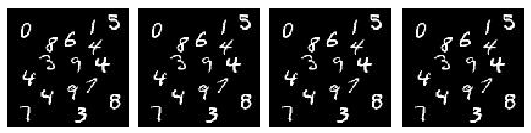
\includegraphics[width=0.9\textwidth]{images/l2cmnist}}
		\caption{An example of even-odd digits images. Form left to right, images contain 0, 5, 10 and 15 even digits.}
	\label{fig:l2cmnist}
\end{figure}

\indent This dataset has in total 1 million images, 800,000 images for training set and 200,000 as the test. Also, the dataset is uniformly generated, meaning that for instance, the number of images containing 0 even digits are equal to the number of images containing 15 even digits.  

\subsection{Synthetic pedestrians dataset}
\label{subsec:synped}
Learning features using deep architectures require a large amount of data. More importantly, for a fully supervised learning, this data should be annotated. Lack of data or its' High annotation cost prohibit the usage of deep learning methods for many problems including Crowd counting. 

\indent However, in order to soften this cost, in our research, we decided to synthetically generate a data set of pedestrians in a walkway. To do that, we used UCSD unlabeled dataset of pedestrians used in \cite{chan2009analysis, mahadevan2010anomaly, li2014anomaly}. UCSD Anomaly detection dataset contains clips of groups of people walking towards and away from the camera, and some amount of perspective distortion. Contains 34 training video samples and 36 testing video samples. Each video has 200 frames of each $238\times158$ pixels.


\indent In our study, we used the 36 testing video samples to generate the synthetic pedestrians dataset. To pore over the generation of our dataset, we divide this process into data generation and data improvement.

  
\subsubsection{Data generation}

In our dataset, we constrained each image by having up to 29 pedestrians in the walkway. The process of generating the data includes the following steps:
\begin{enumerate}

\item \textbf{Background extraction:} Firstly, we simply subtract the background from each video frame. We extract two types of backgrounds, the median of all the backgrounds in each video (in total, 36 different backgrounds), and the median of all median backgrounds.

\item \textbf{Pedestrian extraction:} Subtracting each image from the mean background, we were able to label the connected regions of the subtraction using morphological labeling methods. Then, properties of labeled regions are measured and bound-boxed (see \cite{van2014scikit} for more detailed explanation). Boxes of people are center-based annotated. These labeled boxes shape our initial list of pedestrians with black and white masks of the same size of each box.

\item \textbf{Background generation:} In this step, we tried to make the backgrounds of images as realistic as we could, by first, make a sparse combination of median backgrounds, secondly, changing the global illumination of the images randomly and at last, adding some \textit{Gaussian noise} to the backgrounds. 

\item \textbf{Generating the images:} Having backgrounds generated and pedestrians extracted and labeled, backgrounds are selected randomly. Then, for training and comparison purposes, images are masked with a \textit{Region Of Interest}~(ROI) filter. Afterwards, pedestrians are added to the masked background in a way that the center of each person is placed inside white area of the mask. Finally images are normalized and resized to $158\times158$ in order to be fed to convolution layers

\end{enumerate}

\subsubsection{Data improvement}
Although we managed to successfully generate synthetic images of people in the street, the generated images were still quite distinguishable from the real dataset. Thus, in order to better and enrich images, we improved the dataset in the aspects explained underneath:
\begin{itemize}
\item \textbf{Non-pedestrian objects:} Amongst the extracted boxes of pedestrians, there were some non-pedestrian boxes. Some with objects instead of pedestrians and others with more than one person inside the box. Therefore, we manually removed these outliers. After this edition, we ended with 315 samples of people. 
\item \textbf{Lacking pedestrians:} For the sake of generalization of our model, we needed a decent variety of pedestrians. To that end, we created 3 versions of current pedestrians list, each darkened by the factor of 20\% from each other. 
\item \textbf{Halos around the pedestrians:} Due to lack of accuracy of the region measuring method, a fine layer of the background the pedestrians were extracted from, were still remained around the pedestrians. In the new images, depending on where the person was placed, these thin layer appeared like a halo around the person. To tackle this issue, we tried two approaches:
\begin{enumerate}
\item \textbf{Morphological erosion:} Among morphological operations on image, we applied \textit{erosion} \cite{van2014scikit} to erode the pedestrians masks. In this way, the halos were ignored to some noticeable extent. 
\item \textbf{Poisson image editing:} Poisson image editing is a technique for seamlessly blending two images together fully automatically  \cite{perez2003poisson}. In addition to erosion, we tried Poisson image editing tool to remove the halos. However, due to our gray-scale and low-resolution images, this tool did not have a great impact on our images.      
\end{enumerate}
\item \textbf{Image Perspective:} Since pedestrians of different sizes were put randomly in the images, we considered people's tallness perspective in the images. Human height almost follows a Gaussian distribution \cite{subramanian2011height}. Therefore, with respect to \cite{subramanian2011height, garcia2007evolution}, we mapped individual's heights with the length of the walkway in the image, considering a Gaussian noise with mean $\mu = 0$ and $\sigma = 3.5$.  
\end{itemize}

\noindent Thusly, we created a set of 1 million images, each of size $158\times158$ pixels with up to 29 pedestrians. We assigned 800,000 images for training set and 200,000 instances as the test set. We believe the created synthetic dataset of pedestrians is realistic enough to be able to represent a real-world crowd counting scenario.

\subsection{UCSD crowd counting dataset}
\label{subsec:datareal2}
To verify and validate our model, we used UCSD crowd counting dataset created by \citeauthor*{chan2008privacy} and used in \cite{chan2008privacy,chan2009bayesian,chan2012counting}. The dataset contains video of pedestrians on UCSD walkways, taken from a stationary camera. There are currently two  viewpoints available among which we used \textit{vidf} videos. All videos are 8-bit gray-scale, each video file has 200 video frames, with dimensions $238\times158$. In our experiment, the first 20 videos which are labeled with the number of pedestrians were incorporated. The center point of each pedestrian defines its' location in the image. 

\indent Among the labeled images, we selected the ones in which the number of pedestrians do not exceed 29. Then, images were resized to the dimension $158\times158$ and normalized between 0 and 255. Hence, in total we have a dataset of 3375 real images which are masked with the same filter we used for synthetic pedestrians dataset. 

\indent We will use to first, validate the performance of our model trained with synthetic data, on a real dataset, and also to comparison between work done in \cite{chan2008privacy} and our approach. 